\subsection*{продолжаем}
Давайте посчитаем намагниченность газа диполей
\begin{equation*}
	M^z = - \frac{\partial F}{\partial H} = T N \frac{\partial}{\partial H} \ln(Z_1) = T N \frac{1}{Z_1}\frac{\partial Z_1}{\partial \alpha} \frac{\partial \alpha}{\partial H} = N \mu \frac{1}{Z_1} \frac{\partial Z_1}{\partial \alpha},
\end{equation*}
где $\partial\alpha/\partial H = \mu/T$. Теперь отдельно вычислим
\begin{equation*}
	\frac{1}{ Z_1} \frac{\partial Z_1}{\partial \alpha} = L(\alpha) = \frac{1}{\frac{4 \pi}{\alpha} \sh \alpha} \left[\frac{4 \pi \ch \alpha}{\alpha} - \frac{4 \pi \sh \alpha}{\alpha^2}\right].
\end{equation*}
Тут можно углядеть функцию Ланжевена и переписываем намагниченность
\begin{equation*}
	L(\alpha) = \left[\cth \alpha - \frac{1}{\alpha}\right],
	\hspace{1 cm}
	M^z = N \mu L(\alpha).
\end{equation*}
\begin{figure}[h]
    \centering
    \includegraphics[width=0.5\textwidth]{img/sem4im1.pdf}
    %\caption{}
    %\label{fig:}
\end{figure}

\begin{itemize}
	\item при $\alpha \to 0$: $M^z = \frac{N \mu \alpha}{3} = \frac{N \mu^2 H}{3 t}$, где можно ввести $\chi = \frac{N \mu^2}{3 T} \sim \frac{1}{T}$ -- закон Кюри;
	\item при $\alpha \to \infty$ $M^z = N \mu$.
\end{itemize}

Теперь другим способом, зная что $\langle x\rangle = \int_{-\infty}^{+\infty} x w(x) d x$, то есть
\begin{equation*}
	\langle \mu^z\rangle = \int m^z w(\vc{n}) d \Omega = \int \mu \cos \theta \frac{1}{Z_1} e^{- \varepsilon(\smallvc{n})/T} d \Omega
	=
	\frac{1}{Z_1} \int \mu^z e^{\frac{\mu^z H}{T}} d \Omega = \frac{T}{Z_1} \int \frac{\partial}{\partial H} e^{\frac{\mu^z H}{T}} d \Omega
	=
	\frac{T}{Z_1} \frac{\partial}{\partial H} \int e^{\mu^z H/T} d \Omega
\end{equation*}
\begin{equation*}
	\langle \mu^z\rangle = \frac{T}{Z_1} \frac{\partial}{\partial H} Z_1 = T \frac{\partial}{\partial H} \ln Z_1 = - \frac{\partial}{\partial H} (- T \ln Z_1).
\end{equation*}
Ну и замечаем, что получилась термодинамическая формула вообще
\begin{equation*}
	N \langle \mu^z\rangle = M^z = - \frac{\partial}{\partial H}( - T N \ln Z_1),
	\hspace{1 cm}
	M^z - \frac{\partial F}{\partial H}, 
	\hspace{0.5 cm}
	Z = Z_1^N = - \frac{\partial}{\partial H} F.
\end{equation*}

\subsection*{Квантовый случай}
Теперь будем рассматривать квантовый газ атомов в магнитном поле. Каждый атом имеет собственный момент $J$, проекция которого на ось магнитного поля $z$ будет квантоваться по $\nu = - J, \ldots, + J$.
В магнитном поле они приобретают добавку к энергии $\Delta E_\nu = g_J \mu_\text{Б} H \nu$.
\begin{equation*}
	Z_1 = \sum_{\text{кв. сост.}} e^{\Delta E_\nu /T} = \sum_{\nu = J}^{+J} e^{- \frac{g_J \mu_\text{Б} H \nu}{T}} = \sum_\nu e^{- \alpha \nu} = e^{\alpha J} [1 + e^{- \alpha} + e^{- 2\alpha} + \ldots + e ^{-2 \alpha J}].
\end{equation*}
Получили сумму геометрической прогрессии из $n = 2 J + 1$ элементов.
\begin{equation*}
	Z_1 = e^{\alpha J} \frac{e^{-\alpha (2 J +1)} - 1}{e^{-\alpha} - 1} = \frac{e^{\alpha J} - e^{- \alpha J - \alpha}}{1 - e^{-\alpha}} = \frac{e^{\alpha (J + 1/2)} - e^{- \alpha (J + 1/2)}}{e^{\alpha/2} - e^{-\alpha/2}}.
\end{equation*}
И так получили статсумму
\begin{equation*}
	Z_1 = \frac{\sh \alpha (J+1/2)}{\sh \alpha/2}.
\end{equation*}
И теперь мы знаем всё! Статсумма всей системы
\begin{equation*}
	Z = Z_1^N,
	\hspace{1 cm}
	F = - T \ln Z = - T N \ln Z_1.
\end{equation*}
И намагниченность
\begin{equation*}
	M^z = - \frac{\partial F}{\partial H} = T N \frac{1}{Z_1} \frac{\partial Z_1}{\partial H}
	= T N \frac{1}{Z_1} \frac{\partial Z_1}{\partial \alpha} \frac{\partial \alpha}{\partial H} = T N \frac{g_J \mu_\text{Б}}{T} \frac{1}{Z_1} \frac{\partial Z_1}{\partial \alpha}.
\end{equation*}
Теперь осталось продифференцировать
\begin{equation*}
	\frac{\partial Z_1}{\partial \alpha} = \frac{1}{\frac{\sh \alpha(J+1/2)}{\sh \alpha/2}} \left[\frac{\ch \alpha(J+1/2)}{\sh \alpha/2} ( J + 1/2) - \frac{1}{2} \frac{\ch \alpha/2}{\sh^2 \alpha/2} \sh \alpha (J+1/2)\right]
	=
	(J+1/2) \cth \alpha(J + 1/2) - \frac{1}{2} \cth \alpha/2
	\equiv B_J(\alpha),
\end{equation*}
где $B_J(\alpha)$ -- функция Бриллюэна\footnote{за график спасибо Саше Яворскому.}.
\begin{figure}[h]
    \centering
    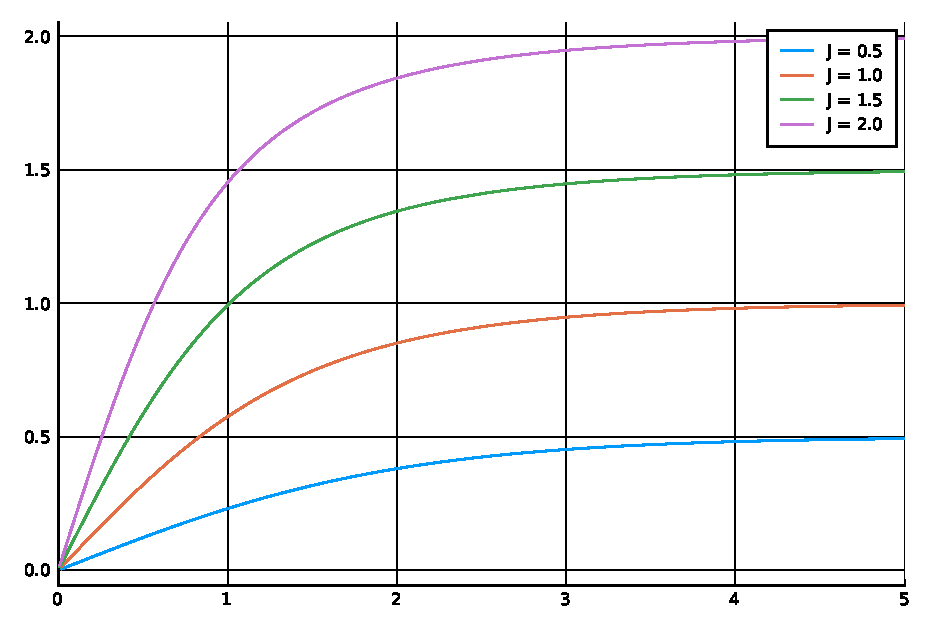
\includegraphics[width=0.6\textwidth]{img/brillouin.eps}
    \caption{График $M^z(\alpha)$. В отрицательную сторону симметрично.}
    %\label{fig:}
\end{figure}
В слабых полях 
\begin{equation*}
	M^z = N g_J \mu_\text{Б} \frac{J(J+1)}{3} \frac{g_J \mu_\text{Б} H}{T} = N \frac{(g_J \mu_\text{Б})^2}{3 T}J (J+1) H.
\end{equation*}
\begin{itemize}
	\item  $g_J m_B H \ll T$ -- слабое поля ($\alpha \ll 0$): $\chi = N \frac{(g_J\mu_\text{Б})^2}{3 T}J (J+1) \sim \frac{1}{T}$ -- закон Кюри;
	\item $g_J m_B H \gg T$ -- сильное поле ($\alpha \gg 0$): $M^{z} = g_J \mu_\text{Б} N J$.
\end{itemize}

\subsection*{Каноническое распределение для классического газа}
Теперь $N$ атомов как-то двигаются в объёме $V$, и задана температура $T$. Реализации такого макросостояния можно добиться по-разному.
\begin{equation*}
	Z = \sum e^{- H(\smallvc{p}_i, \smallvc{r}_i)/T} = \int d \Gamma e^{- H(\smallvc{p}_i, \smallvc{r}_i)/T} 
\end{equation*}
Плотность состояний
\begin{equation*}
	d \Gamma =  \frac{1}{N!}\left(\frac{1}{(2 \pi \hbar)^3}\right)^N d^3 p_1 d^3 r_1 d^3 p_2 d^3 r_2 \ldots d^3 p_N d^3 r_N
	=
	\frac{1}{N!} \frac{\prod_{i = 1}^N d^3 p_i d^3 r_i}{(2 \pi \hbar)^{3N}}.
\end{equation*}
То есть придётся взять интеграл
\begin{equation*}
	Z = \int \frac{1}{N!} \frac{\prod_{i = 1}^N d^3 p_i d^3 r_i}{(2 \pi \hbar)^{3N}} e^{- H(\smallvc{p}_i, \smallvc{r}_i)/T}.
\end{equation*}